\chapter{Helium Interaction with BCC Lithium}
Lithium is becoming an important element in the context of magnetic fusion devices. Lithium-coated surfaces have been tested in several fusion devices in the world~\cite{bell2009plasma, mirnov2003li, sanchez2009impact, tuccillo2009overview, xu2011study, munaretto2012rfx}. There are earlier examples of using lithium in fusion reactors. Erents \etal~\cite{erents1971trapping}\@ used lithium to trap deuterons in solid and liquid lithium. Liquid lithium also proven to be efficient trapper of hydrogen. Lithium reacts with deuterium and forms lithium hydride (LiH), which is ionic in nature. 

Lithium was also proposed as a breeding material in fusion reactors~\cite{hartley1978potential}. For this, lithium needs to be enriched in lithium-6. The recent interest in using solid lithium (applied to a graphite or tungsten surface) in fusion reactors is for density and impurity control in the temperature range of 30--50 \textdegree C~\cite{allain2012lithium}.  In the near surface region of plasma facing materials, high densities of interstitials and vacancies are produced in addition to higher concentration of hydrogen and helium being present. These defects and gases will change the microstructure of the material. It is therefore important to determine the properties of defects in Lithium and their interaction with helium atom. The goal of this study is to calculate some important quantities regarding point defects in lithium and helium in lithium using density functional theory.

\section{Methodology}
We performed all of our calculations using density functional theory (DFT) with plane-wave basis sets as implemented in the software \textsc{QuantumEspresso}\cite{giannozzi2009quantum}. The projector augmented method (paw)~\cite{blochl1994projector} based pseudopotentials from \textsc{QuantumEspresso's} PS library~\cite{dal2014pseudopotentials,pp1} were used. The generalized gradient approximation of Perdew,Burke, and Ernzerhof (PBE) was used as exchange-correlation functional~\cite{Perdew1996b, Perdew1997}. We used a $4\times4\times4$ supercell of bcc lithium, which consists of 128 atoms to simulate defects. Brillouin zone sampling was performed using the scheme of Monkhorst and Pack~\cite{pack1977special} with a $k$-point mesh of $5\times5\times5$. The plane wave cutoff energy was 50 Ry. The equilibrium lattice parameter obtained was 3.436 \AA\@ for bcc lithium. All the calculations were performed at constant volume fully relaxing the atomic positions in the supercell. The migration energies were calculated using the nudged elastic band method~\cite{henkelman2000climbing, henkelman2000improved} with seven images along the migration pathway.

The formation energies are calculated as follows:
\begin{align}\label{eq_forme}
\begin{split}
 E_{f}^{\text{oct}} & = E_{\text{Li}+\text{He}_{\text{oct}}} - E_{\text{Li}_N} - E_{\text{He}_{\text{isolated}}} \\
 E_{f}^{\text{tetr}}& = E_{\text{Li}+\text{He}_{\text{tetr}}} - E_{\text{Li}_N} - E_{\text{He}_{\text{isolated}}} \\
 E_f^{\Box} & = E_{\text{Li}_{N-1}} - \frac{N-1}{N} E_{\text{Li}_N} \\
 E_f^{\text{subs}} & = E_{\text{Li}+\text{He}_{\Box}} - \frac{N-1}{N} E_{\text{Li}_N} - E_{\text{He}_{\text{isolated}}}
\end{split}
 \end{align}
\nomenclature{$E_f^{\text{subs}}$}{helium formation energy in a substitutional position}
\nomenclature{$E_f^{\text{tetr}}$}{helium formation energy in a tetrahedral position}
\nomenclature{$E_f^{\text{oct}}$}{helium formation energy in a octahedral position}
\nomenclature{$E_{\text{He}_{\text{isolated}}}$}{energy of an isolated helium atom}
Here, $E_{\text{Li}+\text{He}_{\text{tetra/octa}}}$ is the energy of a system in which helium is at either octahedral or tetrahedral sites in bcc lithium. $E_{\text{Li}+\text{He}_{\Box}}$ is the energy of a system in which helium is in a substitutional position. $E_{\text{Li}_N}$ is the energy of defect free lithium, and $E_{\text{He}_{\text{isolated}}}$ is the energy of an isolated helium atom. $E_{\text{Li}_{N-1}}$ is the energy of a lithium bcc supercell with a vacancy.


The formation energy of an self-interstitial atom (SIA) is calculated using
\begin{equation}
E_f^{\text{SIA}} = E_{\text{Li}_{N+1}} - \frac{N+1}{N} E_{\text{Li}_N}
\end{equation}
where, $E_{\text{Li}_{N+1}}$ is the energy of a system with a self interstitial (Li) atom in either an octahedral or tetrahedral position.
The binding energies of two helium atoms is determined as obtained as: 
\begin{equation}
E_{\text{b}}^{\text{He}_1\text{--}\text{He}_2} = E_{\text{Li}+\text{He}_1} + E_{\text{Li}+\text{He}_2} - E_{\text{Li}_N+\text{He}_1 + \text{He}_2} - E_{\text{Li}_N} 
\end{equation}
here, $E_{\text{Li}_N}$ is the energy of the supercell without any helium present, $E_{\text{Li}+\text{He}_1/\text{He}_2}$ is the energy of the supercell with a single helium interstitial.  $E_{\text{Li}_N+\text{He}_1 + \text{He}_2}$ is the energy of the supercell containing two nearby helium atoms. For more than two helium atoms, the following equation is used to calculate the binding energies between them.
\begin{equation}
E_b^{\text{He}_n} = \sum_{i=1,\dots,n} E_{\text{Li}_N+\text{He}_i} - \left[ E_{\text{Li}_N+\text{He}_n} + (n-1)E_{\text{Li}_N} \right ]
\end{equation}
The helium--helium dumbbell formation energy (two helium atoms sharing a vacancy) can be calculated using the following equation:
\begin{equation}\label{eq_hedmbl}
E_f^{\text{He}-\Box-\text{He}} = E_{\text{Li}_{N-1}+\text{He}-\Box-\text{He}} - E_{\text{Li}_N} + \frac{E_{\text{Li}_N}}{N} - E_{\text{He}_{\text{isolated}}}
\end{equation}
\nomenclature{$E_f^{\text{He}-\Box-\text{He}}$}{helium--helium dumbbell formation energy around a vacancy}
Here, $E_{\text{Li}_{N-1},\text{He}-\Box-\text{He}}$ is the energy of a supercell containing the helium dumbbell.

\section{Results and Discussion}
We have calculated the formation energies for different configurations of the self-interstitial atoms and the vacancy formation energy for lithium. The results are presented in Table~\ref{tab:lidmble}. Our results are comparable with previous DFT calculations and with experiments. The earlier DFT studies produced formation energies of lithium self vacances from 0.52--0.57 eV~\cite{benedek1992formation, Pawellek_1991, frank1993properties, frank1996first}. Compared to our value of 0.496 eV the discrepancy could come from the size of the supercell, elastic interaction, and the quality of the pseudopotential. 

We also calculated the self-interstitial formation energy in lithium. Octahedral self-interstitial are unstable and relaxes to a dumbbell oriented in \hkl<010> directions. Tetrahedral interstitials are also unstable and relaxes to \hkl<110> dumbbells. The lowest energy dumbbell orientation are the \hkl<111> orientations, which is a similar trend as in other nonferro-magnetic bcc materials. The vacancy formation energy is slightly lower than Frank \etal~\cite{frank1996first} and Ma and Dudarev~\cite{ma2019effect}, while the migration energy of the vacancy in \hkl<111> direction is slightly higher than Ma and Dudarev~\cite{ma2019effect}. The self-interstitial dumbbell formation energy is comparable to the values reported by Ma and Dudarev~\cite{ma2019}.

\begin{table}
\caption[Calculated vacancy formation energy $E_f^{\Box}$, vacancy migration energy, and self-interstitial formation energy in lithium]{Calculated vacancy formation energy $E_f^{\Box}$, vacancy migration energy, and self-interstitial formation energy in lithium. Calculated results are compared with some of the previous work and experimental results (in italics).}
\label{tab:lidmble}
\centering
\begin{minipage}{28.5em}
\let\footnoterule\relax
\begin{tabular}{c c c} \toprule
Defect					& Formation Energy (eV)						& Previous Work \\ \midrule
						&											& 0.52~\cite{frank1996first} \\ 
vacancy ($E_f^{\Box}$)	& 0.496										& 0.506~\cite{ma2019effect} \\
						&										& \textit{0.508}~\cite{LandoltBornstein1991} \\ \hline
\hkl<111>			   & 0.589										&  0.573~\cite{ma2019}	 \\ \hline
\hkl<110>\footnote{equivalent to tetrahedral SIA formation}   & 0.646 & 0.637~\cite{ma2019}	 \\ \hline
\hkl<010>\footnote{equivalent to octahedral SIA formation}   & 0.791 &  0.782~\cite{ma2019}    \\ \hline
tetrahedral ($E_f^{\text{tetr}}$) &	0.646 &	0.696~\cite{ma2019}	\\ \hline
octahedral ($E_f^{\text{oct}}$) & 0.793	& 0.785~\cite{ma2019}	\\ \hline
Vacancy migration energy       & 0.086 & 0.053~\cite{ma2019effect}	\\ 
							   &       & \textit{0.038}~\cite{LandoltBornstein1991} \\ 
\bottomrule
\end{tabular}
\end{minipage}
\end{table}


\begin{table}
\caption[Formation energies (in eV) for a single helium atom positioned in the octahedral or tetrahedral interstitial sites as well as in substitutional site]{Formation energies (in eV) for a single helium atom positioned in the octahedral or tetrahedral interstitial sites as well as in substitutional site. Helium migration energy (eV) from one interstitial site to next interstitial site. The Calculations are done using 128 atom supercells. The results are compared with helium interaction with tungsten and iron which are both bcc material at standard temperature and pressure.}
\label{tab:he_li} 
\centering
\renewcommand{\arraystretch}{1.45}
\begin{tabular}{c c c c} \toprule
Configuration   & Li--He  &  W--He~\cite{becquart2007ab}   &  Fe--He~\cite{seletskaia2005magnetic} \\ \midrule
$E^{f}_{\text{oct}}$  & 1.142   &  6.38    & 4.60   \\ \hline
$E^{f}_{\text{tetr}}$ & 1.132   &  6.16    & 4.37   \\ \hline
$E^f_{\text{subs}}$          & 1.213   &  4.70    & 4.08   \\ \hline
$E^{t-t}_{\text{mig}}$       & 0.003   &  0.06    & 0.06    \\ \hline 
$E^{t-o-t}_{\text{mig}}$     & 0.013   &		   &		\\ \hline
$E^{o-o}_{\text{mig}}$		  & 0.004  &			&		\\ \hline
$E^{\text{He}-\text{He}}_b$   & 0.209  &  1.03		 &		\\ 
	\bottomrule
\end{tabular}
\end{table}

\begin{table}
\caption{Formation of  He--He dumbbells around a vacancy}
\label{tab:hedmble}
\centering
\begin{tabular}{c c} \toprule
Dumbbell Configuration & Formation Energy (eV) \\ \midrule
\hkl<111>   & 1.844 \\ \hline
\hkl<110>   & 1.863  \\ \hline
\hkl<010>   & 1.879 \\ 
\bottomrule
\end{tabular}
\end{table}

During the operation of the fusion reactor, the lithium-coated surface will interact with high fluxes of different hydrogen isotopes and helium plasmas. This could initiate neutron-activated reactions and transmute lithium to hydrogen and helium. All of these processes will build up a substantial amount of hydrogen and helium inside the material. Significant research has been and is still being performed to understand the behaviour of helium in metals. 

One of the major challenges is the low solubility of helium in metals. Helium atoms in a metal may find low-energy positions either in substitutional or interstitial lattice sites. We calculated the formation energies of different configurations of helium in substitutional as well as interstitial positions using Eq.~\eqref{eq_forme}. The results are presented in Table~\ref{tab:he_li}. We compare our results to similar energies in tungsten and iron. Our calculation predicts that the tetrahedral interstitial position is the lowest energy for helium, which is also the case for tungsten and iron~\cite{becquart2007ab,fu2005}. The difference between the octahedral and tetrahedral interstitial formation energy is only 0.01 eV. This is very low compared to tungsten--helium (0.22 eV) and iron--helium (0.23 eV). The formation energy of helium in a substitutional location is 1.213 eV. This value is higher than both tetrahedral and the octahedral interstitial formation energies. This is an atypical result compared compared to other bcc metals, for which the substitutional site has a significantly lower formation energy than the two interstitial sites. We reproduced this result using different DFT package (\ie, \textsc{Abinit~\cite{gonze2016, gonze2020}}) and also got a similar value using  ultrasoft pseudopotential. 
\begin{figure}
\centering
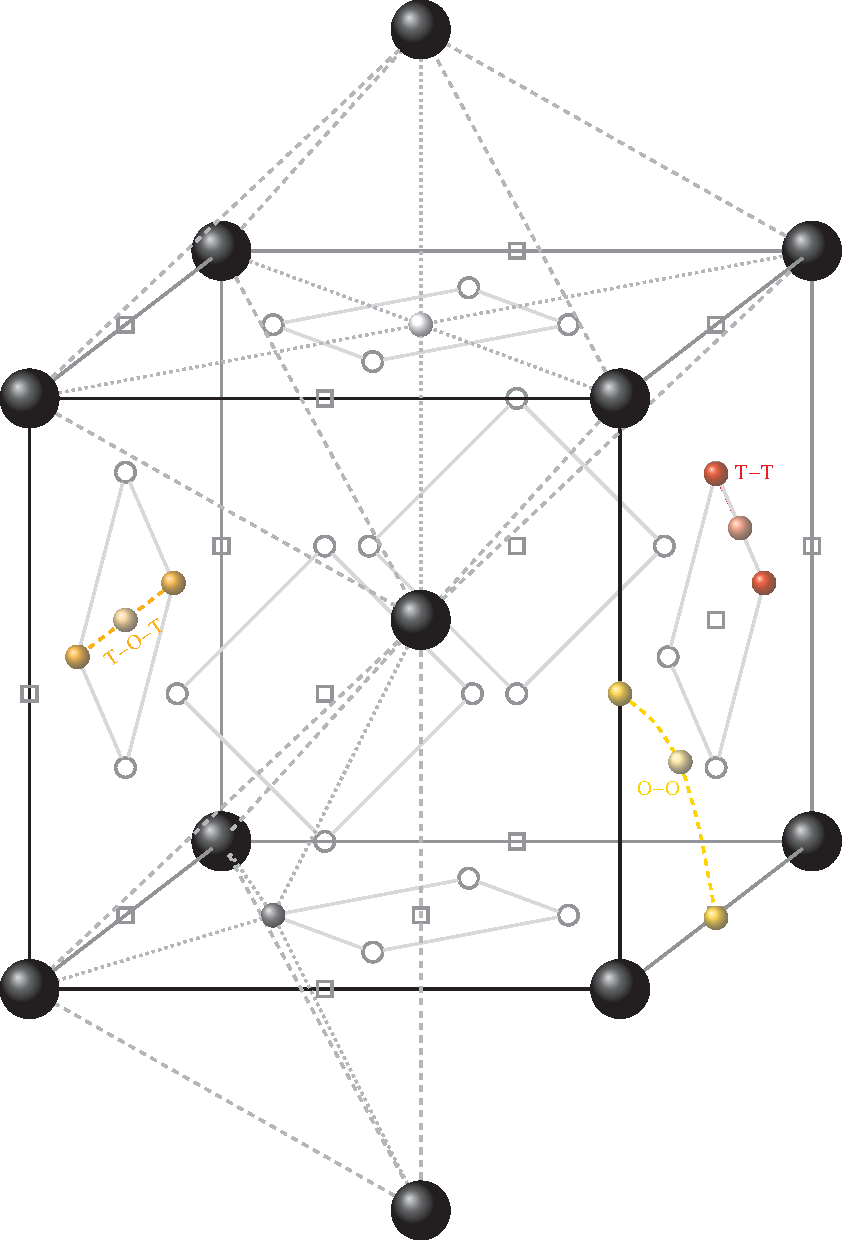
\includegraphics[scale=0.7]{bcc-sites}
\caption{Tetrahedral $(\circ)$ and octahedral $(\Box)$ interstitial positions in bcc crystal. Three different migration paths: Tetrahedral to tetrahedral (T-T), octahedral to octahedral (O-O), and tetrahedral to octahedral to tetrahedral (T-O-T).}
\label{fig:dmbl}
\end{figure}

\begin{figure}
\centering
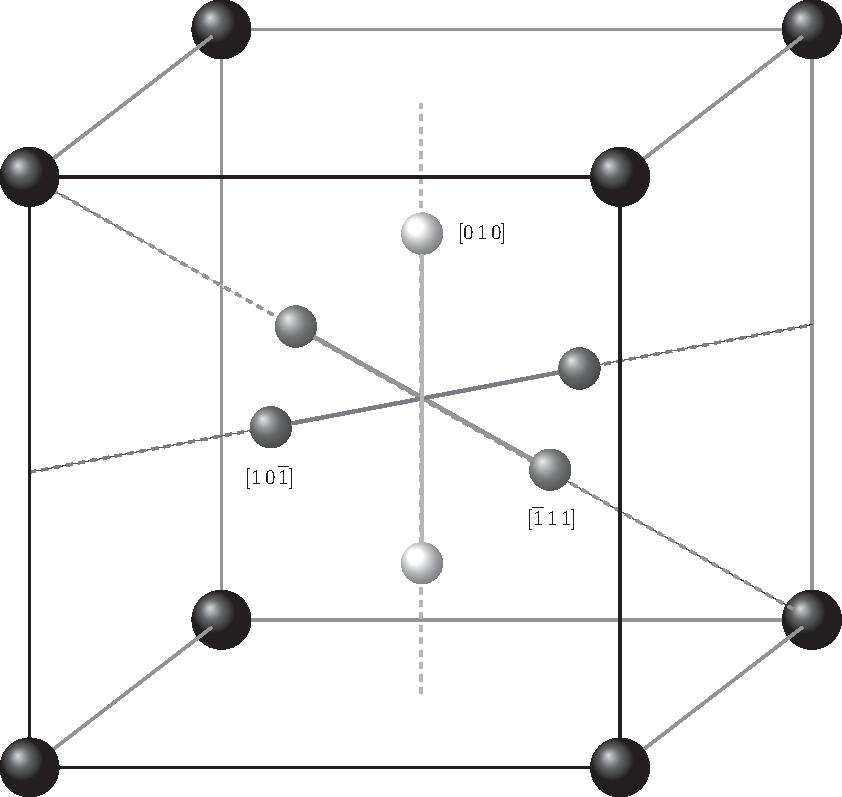
\includegraphics[scale=0.7]{bcc-dumbbells}
%\caption{Tetrahedral (t) and octahedral (o) site on the (001) plane of the bcc lattice.}
\caption{Different dumbbell configurations in bcc crystal.}
\label{fig:001}
\end{figure}

We also calculated the binding energy of helium to a vacancy. Even though, the substitutional energy is higher, a single helium at interstitial site still finds its place on a nearby vacancy. The binding energy of helium in a substitutional position to a vacancy is 0.21 eV. The binding energy of helium in a tetrahedral interstitial location and a vacancy is 0.42 eV. The binding energy between two helium atoms at nearby interstitial sites is 0.208 eV, which is lower than tungsten--helium system. Binding energy of multiple helium atoms to a vacancy is calculated. The result is shown in Fig.~\ref{fig:he-bind}. It shows almost a linear increase of binding energy around a vacancy. Which indicates that a group of helium atom tend to aggregate to vacancy. 

Two helium atoms around a vacancy form a dumbbell much like lithium self-interstitials do. The formation energies vary based on the orientation of the dumbbell. The helium dumbbell formation energies are presented in Table~\ref{tab:hedmble}. The lowest-energy orientations are \hkl<111> directions. The migration energies of helium from one tetrahedral site to a nearby tetrahedral site (Fig.~\ref{fig:001}) were the calculated using nudged elastic band method. The calculated energy from one tetrahedral site to a next tetrahedral site (Fig.~\ref{fig:001}) is 0.003 eV. Tungsten--helium and iron--helium have a slightly higher migration energy ($E_{mig}^{t-t}$) of 0.006 eV. The migration energy from one octahedral site to the next octahedral site is 0.004, which is also very low. The low migration energies indicate that helium would be highly mobile inside the matrix.


\begin{figure}
\centering
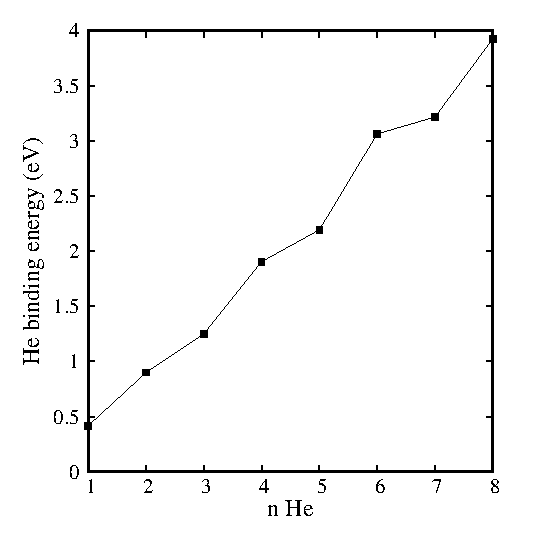
\includegraphics[scale=1.2]{he-vac-bind-E}
\caption{Helium binding energy around a vacancy}
\label{fig:he-bind}
\end{figure}


\clearpage
\bibliographystyle{apsrev4-2}
\bibliography{abbreviated,final}
%\bibliography{abbreviated,lihe}
